\chapter{Introduction to data}
\label{introductionToData}
\label{ch_intro_to_data}

%\begin{tipBox}{\tipBoxTitle[Chapter Goal:]{Thinking about data}
%Understand basics about data organization, data types, numerical summaries of data, graphical summaries of data, and foundational techniques for data collection. We begin and end the chapter with case studies.}
%\end{tipBox}

Scientists seek to answer questions using rigorous methods and careful observations. These observations -- collected from the likes of field notes, surveys, and experiments -- form the backbone of a statistical investigation and are called \term{data}. Statistics is the study of how best to collect, analyze, and draw conclusions from data. It is helpful to put statistics in the context of a general process of investigation:
\begin{enumerate}
\setlength{\itemsep}{0mm}
\item Identify a question or problem.
\item Collect relevant data on the topic.
\item Analyze the data.
\item Form a conclusion.
%\item Make decisions based on the conclusion.
\end{enumerate}
Statistics as a subject focuses on making stages 2-4 objective, rigorous, and efficient. That~is, statistics has three primary components: How best can we collect data? How should it be analyzed? And what can we infer from the analysis?

The topics scientists investigate are as diverse as the questions they ask. However, many of these investigations can be addressed with a small number of data collection techniques, analytic tools, and fundamental concepts in statistical inference. This chapter provides a glimpse into these and other themes we will encounter throughout the rest of the book. We introduce the basic principles of each branch and learn some tools along the way. We will encounter applications from other fields, some of which are not typically associated with science but nonetheless can benefit from statistical study.

\section[Case study: using stents to prevent strokes]{Case study: using stents to prevent strokes \sectionvideohref{youtube-nEHFF1ADpWE&list=PLkIselvEzpM6pZ76FD3NoCvvgkj_p-dE8} \sectionslideshref{gdoc_os3_slides_1-1}}
\label{basicExampleOfStentsAndStrokes}

\index{data!stroke|(}

Section~\ref{basicExampleOfStentsAndStrokes} introduces a classic challenge in statistics: evaluating the efficacy of a medical treatment. Terms in this section, and indeed much of this chapter, will all be revisited later in the text. The plan for now is simply to get a sense of the role statistics can play in practice.

In this section we will consider an experiment that studies effectiveness of stents in treating patients at risk of stroke.\footnote{Chimowitz MI, Lynn MJ, Derdeyn CP, et al. 2011. Stenting versus Aggressive Medical Therapy for Intracranial Arterial Stenosis. New England Journal of Medicine 365:993-1003. \oiRedirect{textbook-nejm_stent_study}{www.nejm.org/doi/full/10.1056/NEJMoa1105335}. NY Times article reporting on the study: \oiRedirect{textbook-nytimes_stent_study}{www.nytimes.com/2011/09/08/health/research/08stent.html}.} Stents are devices put inside blood vessels that assist in patient recovery after cardiac events and reduce the risk of an additional heart attack or death. Many doctors have hoped that there would be similar benefits for patients at risk of stroke. We start by writing the principal question the researchers hope to answer:
\begin{quote}
Does the use of stents reduce the risk of stroke?
\end{quote}

The researchers who asked this question collected data on 451 at-risk patients. Each volunteer patient was randomly assigned to one of two groups:
\begin{itemize}
\item[]\termsub{Treatment group}{treatment group}. Patients in the treatment group received a stent and medical management. The medical management included medications, management of risk factors, and help in lifestyle modification.
\item[]\termsub{Control group}{control group}. Patients in the control group received the same medical management as the treatment group, but they did not receive stents.
\end{itemize}
Researchers randomly assigned 224 patients to the treatment group and 227 to the control group. In this study, the control group provides a reference point against which we can measure the medical impact of stents in the treatment group.

Researchers studied the effect of stents at two time points: 30~days after enrollment and 365~days after enrollment. The results of 5 patients are summarized in Figure~\ref{stentStudyResultsDF}. Patient outcomes are recorded as ``stroke'' or ``no event'', representing whether or not the patient had a stroke at the end of a time period.

\begin{figure}[h]
\centering
\begin{tabular}{l ccc}
\hline
Patient	&	group	&	0-30 days 	&	0-365 days \\
\hline
1		&	treatment &	no event &	no event \\
2		&	treatment &	stroke & stroke \\
3		&	treatment &	no event & no event \\
$\vdots$	&	$\vdots$	  &	$\vdots$ \\
450	&	control &	no event &	no event \\
451	&	control &	no event &	no event \\
\hline
\end{tabular}
\caption{Results for five patients from the stent study.}
\label{stentStudyResultsDF}
% trmt <- c(rep('trmt', 224), rep('control', 227)); outcome30 <- c(rep(c('event', 'no_event'), c(33, 191)), rep(c('event', 'no_event'), c(13, 214))); outcome365 <- c(rep(c('event', 'no_event'), c(33, 191)), rep(c('event', 'no_event'), c(13, 214)))
\end{figure}

Considering data from each patient individually would be a long, cumbersome path towards answering the original research question. Instead, performing a statistical data analysis allows us to consider all of the data at once. Figure~\ref{stentStudyResults} summarizes the raw data in a more helpful way. In this table, we can quickly see what happened over the entire study. For instance, to identify the number of patients in the treatment group who had a stroke within 30 days, we look on the left-side of the table at the intersection of the treatment and stroke: 33.

\begin{figure}[h]
\centering
\begin{tabular}{l cc c cc}
& \multicolumn{2}{c}{0-30 days} &\hspace{5mm}\ & \multicolumn{2}{c}{0-365 days} \\
  \cline{2-3} \cline{5-6}
	& 	stroke 	& no event && 	stroke 	& no event \\
  \hline
treatment 	& 33		& 191	&&	45 	& 179 \\
control 		& 13		& 214	&& 	28	& 199 \\
  \hline
Total				& 46		& 405	&&	73	& 378 \\
  \hline
\end{tabular}
\caption{Descriptive statistics for the stent study.}
\label{stentStudyResults}
\end{figure}

\begin{exercise}
Of the 224 patients in the treatment group, 45 had a stroke by the end of the first year. Using these two numbers, compute the proportion of patients in the treatment group who had a stroke by the end of their first year. (Please note: answers to all Guided Practice exercises are provided using footnotes.)\footnote{The proportion of the 224 patients who had a stroke within 365 days: $45/224 = 0.20$.}
\end{exercise}

We can compute summary statistics from the table. A \term{summary statistic} is a single number summarizing a large amount of data.\footnote{Formally, a summary statistic is a value computed from the data. Some summary statistics are more useful than others.} For instance, the primary results of the study after 1~year could be described by two summary statistics: the proportion of people who had a stroke in the treatment and control groups.
\begin{itemize}
\setlength{\itemsep}{0mm}
\item[] Proportion who had a stroke in the treatment (stent) group: $45/224 = 0.20 = 20\%$.
\item[] Proportion who had a stroke in the control group: $28/227 = 0.12 = 12\%$.
\end{itemize}
These two summary statistics are useful in looking for differences in the groups, and we are in for a surprise: an additional 8\% of patients in the treatment group had a stroke! This is important for two reasons. First, it is contrary to what doctors expected, which was that stents would \emph{reduce} the rate of strokes. Second, it leads to a statistical question: do the data show a ``real'' difference between the groups?

This second question is subtle. Suppose you flip a coin 100 times. While the chance a coin lands heads in any given coin flip is 50\%, we probably won't observe exactly 50 heads. This type of fluctuation is part of almost any type of data generating process. It is possible that the 8\% difference in the stent study is due to this natural variation. However, the larger the difference we observe (for a particular sample size), the less believable it is that the difference is due to chance. So what we are really asking is the following: is the difference so large that we should reject the notion that it was due to chance?

While we don't yet have our statistical tools to fully address this question on our own, we can comprehend the conclusions of the published analysis: there was compelling evidence of harm by stents in this study of stroke patients.

\textbf{Be careful:} do not generalize the results of this study to all patients and all stents. This study looked at patients with very specific characteristics who volunteered to be a part of this study and who may not be representative of all stroke patients. In addition, there are many types of stents and this study only considered the self-expanding Wingspan stent (Boston Scientific). However, this study does leave us with an important lesson: we should keep our eyes open for surprises.

\index{data!stroke|)}

\section[Data basics]{Data basics \sectionvideohref{youtube-Mjif8PTgzUs&list=PLkIselvEzpM6pZ76FD3NoCvvgkj_p-dE8} \sectionslideshref{gdoc_os3_slides_1-2}}
\label{dataBasics}

Effective presentation and description of data is a first step in most analyses. This section introduces one structure for organizing data as well as some terminology that will be used throughout this book.

\subsection{Observations, variables, and data matrices}

\Comment{This entire section and its data were overhauled.
  The most prominent conspicuous change was removing the
  \data{email50} data set for the \data{loan50} data set.}

\index{data!loan50|(}

Figure~\ref{loan50DF} displays rows 1, 2, 3, and 50 of a data set
for 50 randomly sampled loans offered through Lending
Club over \Comment{list the time period}\footnote{need
to add a citation},
which is \Comment{describe Lending Club}.
These observations will be referred to as the \data{loan50} data set, and they are a random sample from a larger data set that we will see in Section~\ref{}.
\Comment{Need to fill out refs in this paragraph.}

%Figure~\ref{email50DF} displays rows 1, 2, 3, and 50 of a data set concerning 50 emails received during early 2012. These observations will be referred to as the \data{email50} data set, and they are a random sample from a larger data set that we will see in Section~\ref{categoricalData}.

Each row in the table represents a single loan.
The formal name for a row is a \term{case}
or \term{observational unit}\index{unit of observation}.
\Comment{Make unit of observation index point to observational unit.}
The columns represent characteristics,
called \termsub{variables}{variable},
for each of the loans.
For example, the first row represents represents a loan of \$7,500 with an interest rate of 7.34\%, where the borrower is based in Maryland (MD) and has an income of \$70,000. However, while the income source is verified, the amount was not verified.

\begin{exercise}
What is the grade of the first loan in Figure~\ref{loan50DF}?
And what is the home ownership status of the borrower
for that first loan?
You can check your answer in the
footnote.\footnote{The loan's grade is A,
  and the borrower rents their residence.}
\end{exercise}

In practice, it is especially important to ask clarifying
questions to ensure important aspects of the data are understood.
For instance, it is always important to be sure we know what
each variable means and the units of measurement.
Descriptions of the \data{loan50} variables are described
in Figure~\ref{loan50Variables}.

\begin{figure}[h]
\centering
{\small
\begin{tabular}{ccc ccc cc} %c}
  \hline
   & \var{loan\_\hspace{0.3mm}amount}
   & \var{interest\_\hspace{0.3mm}rate}
   & \var{term} & \var{grade} & \var{state}
   & \var{total\_\hspace{0.3mm}income}
   & \var{homeownership} \\ % & verified\_income \\ 
  \hline
  1 & 7500 & 7.34 & 36 & A & MD & 70000 & RENT \\ % & Source Verified \\ 
  2 & 25000 & 9.43 & 60 & B & OH & 254000 & MORTGAGE \\ % & Not Verified \\ 
  3 & 14500 & 6.08 & 36 & A & MO & 80000 & MORTGAGE \\ % & Not Verified \\ 
  $\vdots$ & $\vdots$ & $\vdots$ & $\vdots$ & $\vdots$ & $\vdots$
      & $\vdots$ & $\vdots$ \\ % & $\vdots$ \\
  50 & 3000 & 7.96 & 36 & A & CA & 34000 & RENT \\ % & Not Verified \\ 
   \hline
\end{tabular}
}
\caption{Four rows from the \data{loan50} data matrix.}
\label{loan50DF}
\end{figure}
% Dropped: state, verified_income
% library(openintro); vars <- c("loan_amount", "interest_rate", "term", "grade", "total_income", "home_ownership", "loan_status"); library(xtable); data(loan50); loan50[c(1,2,3,50), vars]; xtable(loan50[c(1,2,3,50), vars])

\begin{figure}[h]
\centering\small
\begin{tabular}{lp{10.5cm}}
\hline
{\bf variable} & {\bf description} \\
\hline
\var{loan\_\hspace{0.3mm}amount} & Amount of the loan received,
    in US dollars.  \\
\var{interest\_\hspace{0.3mm}rate} & Interest rate on the loan,
    in a percent.  \\
\var{term} & The length of the loan, which is always set
    as a whole number of months. \\
\var{grade} & Loan grade, which takes a values A through G
    and represents the quality of the loan and its likelihood
    of being repaid.  \\
\var{state} & US state where the borrower resides. \\
\var{total\_\hspace{0.3mm}income} & Borrower's total income,
    including any second income, in US dollars.   \\
\var{homeownership} & Indicates whether the
    person owns, owns but has a mortgage, or rents.  \\
%\var{verified\_\hspace{0.3mm}income} & Indicates whether the
%    income is verified, its source is verified but not the amount,
%    or it is not verified.   \\
\hline
\end{tabular}
\caption{Variables and their descriptions for the \data{email50} data set.}
\label{loan50Variables}
\end{figure}

\index{data!loan50|)}

The data in Figure~\ref{loan50DF} represent a \term{data matrix},
which is a convenient and common way to organize data,
especially if collecting data in a spreadsheet.
Each row of a data matrix corresponds to a unique case,
and each column corresponds to a variable.
%A data matrix for the stroke study introduced in
%Section~\ref{basicExampleOfStentsAndStrokes} is shown
%in Table~\vref{stentStudyResultsDF}, where the cases were
%patients and three variables were recorded for each
%patient.

When recording data, use a data matrix unless you have
a very good reason to use a different structure.
By using this structure, it is easy to add new cases
as new rows or new variables as new columns.

\begin{exercise}
The grades for assignments, quizzes, and exams in a course are
often recorded in a gradebook that takes the form of a data matrix.
How might you organize grade data using a data
matrix?\footnote{There are multiple strategies that can be followed.
  One common strategy is to have each student represented by a row,
  and then add a column for each assignment, quiz, or exam.
  Under this setup, it is easy to review a single line to understand
  a student's grade history.
  Note that it is also necessary to include additional columns to
  list student information, such as one column to list each student's
  name.}
\end{exercise}

\index{data!county|(}

\begin{exercise}\label{desc_county_as_data_matrix}
We consider data for 3,139 counties in the United States,
which includes each county's name,
the state where it resides, its population,
how its population changed from 2010 to 2017,
poverty rate,
and six additional characteristics.
How might these data be organized in
a data matrix?\footnote{Each county may be viewed as a case,
  and there are eleven pieces of information recorded for
  each case.
  A table with 3,139 rows and 11 columns could hold these data,
  where each row represents a county and each column represents
  a particular piece of information.}
\end{exercise}

\noindent The data described in Guided
Practice~\ref{desc_county_as_data_matrix} represents the
\data{county} data set, which is shown as a data matrix
in Figure~\ref{countyDF}.
The variables are summarized in Figure~\ref{countyVariables}.
\Comment{These data were collected from the US Census website. Move this reference to an appendix.}\footnote{\oiRedirect{textbook-census_quick_facts}{quickfacts.census.gov/qfd/index.html}}

\begin{landscape}
\begin{figure}
\centering\small
\begin{tabular}{ccc ccc ccc ccc}
  \hline
 & \var{name} & \var{state} & \var{pop} & \var{pop\_\hspace{0.3mm}change} & \var{poverty} & \var{homeownership} & \var{multi\_\hspace{0.3mm}unit} & \var{unemp\_\hspace{0.3mm}rate} & \var{metro} & \var{median\_\hspace{0.3mm}edu} & \var{median\_\hspace{0.3mm}hh\_\hspace{0.3mm}income} \\ 
  \hline
  1 & Autauga  & Alabama &  55504 &  1.48 & 13.5 & 77.5 &  7.2 & 3.86 & yes & some\_college & 54487 \\ 
  2 & Baldwin  & Alabama & 212628 &  9.19 & 11.7 & 76.7 & 22.6 & 3.99 & yes & some\_college & 56460 \\ 
  3 & Barbour  & Alabama &  25270 & -6.22 & 29.9 & 68.0 & 11.1 & 5.90 & no  & hs\_diploma   & 32884 \\ 
  4 & Bibb     & Alabama &  22668 &  0.73 & 20.1 & 82.9 &  6.6 & 4.39 & yes & hs\_diploma   & 43079 \\ 
  5 & Blount   & Alabama &  58013 &  0.68 & 14.1 & 82.0 &  3.7 & 4.02 & yes & hs\_diploma   & 47213 \\ 
  6 & Bullock  & Alabama &  10309 & -2.28 & 32.6 & 76.9 &  9.9 & 4.93 & no  & hs\_diploma   & 34278 \\ 
  7 & Butler   & Alabama &  19825 & -2.69 & 24.8 & 69.0 & 13.7 & 5.49 & no  & hs\_diploma   & 35409 \\ 
  8 & Calhoun  & Alabama & 114728 & -1.51 & 17.1 & 70.7 & 14.3 & 4.93 & yes & some\_college & 41778 \\ 
  9 & Chambers & Alabama &  33713 & -1.20 & 19.9 & 71.4 &  8.7 & 4.08 & no  & hs\_diploma   & 39530 \\ 
  10 & Cherokee & Alabama &  25857 & -0.60 & 16.8 & 77.5 &  4.3 & 4.05 & no  & hs\_diploma   & 41456 \\ 
  $\vdots$ & $\vdots$ & $\vdots$ & $\vdots$ & $\vdots$ & $\vdots$ & $\vdots$ & $\vdots$ & $\vdots$ & $\vdots$ & $\vdots$ & $\vdots$ \\
  3143 & Weston & Wyoming &  &  & 10.7 & 77.9 & 6.5 & 3.98 & no & some\_college & 56582 \\ 
   \hline
\end{tabular}
\caption{Eleven rows from the \data{county} data set.}
\label{countyDF}
% library(openintro); data(county); county$name <- gsub(" County$", "", county$name); county$pop <- county$pop2017; county$unemp_rate = county$unemployment_rate; these <- c("name", "state", "pop", "pop_change", "poverty", "home_ownership", "multi_unit", "unemp_rate", "metro", "median_edu", "median_hh_income"); county <- county[, these]; library(xtable); xtable(as.data.frame(lapply(rbind.data.frame(head(county, 10), tail(county, 1)), function(x) { format(x) })))
\end{figure}

\begin{figure}
\centering\small
\begin{tabular}{lp{11cm}}
\hline
{\bf variable} & {\bf description} \\
\hline
\var{name} & County name \\
\var{state} & State where the county resides,
    or the District of Columbia \\
\var{pop} & Population in 2017 \\
\var{pop\_\hspace{0.3mm}change} & Population change from 2010 to 2017 \\
\var{poverty}  &  Percent of the population in poverty \\
\var{homeownership}  &
    Percent of the population that lives in their own home
    or lives with the owner, e.g. children living with parents
    who own the home \\
\var{multi\_\hspace{0.3mm}unit}  &
    Percent of living units that are in multi-unit structures,
    e.g. apartments \\
\var{unemp\_\hspace{0.3mm}rate} & Unemployment rate \\
\var{metro} & Whether the county contains a metropolitan area \\
\var{median\_\hspace{0.3mm}edu} & Median education level, which
    can take a value among
    \resp{below\_\hspace{0.3mm}hs},
    \resp{hs\_\hspace{0.3mm}diploma},
    \resp{some\_\hspace{0.3mm}college},
    and \resp{bachelors} \\
\var{median\_\hspace{0.3mm}hh\_\hspace{0.3mm}income} &
    Median household income for the county, where a household's
    income equals the total income of its occupants who are
    15~years or older \\
\hline
\end{tabular}
\centering
\caption{Variables and their descriptions for the \data{county} data set.}
\label{countyVariables}
\end{figure}
\end{landscape}

\subsection{Types of variables}
\label{variableTypes}

Examine the \var{unemp\_\hspace{0.3mm}rate}, \var{pop}, \var{state},
and \var{median\_\hspace{0.3mm}edu} variables in the \data{county}
data set. Each of these variables is inherently different from the
other three, yet some share certain characteristics.

First consider \var{unemp\_\hspace{0.3mm}rate},
which is said to be a \term{numerical} variable since
it can take a wide range of numerical values,
and it is sensible to add, subtract, or take averages
with those values.
On the other hand, we would not classify a variable
reporting telephone area codes as numerical since their
average, sum, and difference have no clear meaning.

The \var{pop} variable is also numerical, although it seems
to be a little different than \var{unemp\_\hspace{0.3mm}rate}.
This variable of the population count can only take whole
non-negative numbers (\resp{0}, \resp{1}, \resp{2}, ...).
For this reason, the population variable is said to be
\term{discrete} since it can only take numerical values
with jumps.
On the other hand, the poverty rate variable is said
to be \term{continuous}.

The variable \var{state} can take up to 51 values after
accounting for Washington, DC: \resp{AL}, ..., and \resp{WY}.
Because the responses themselves are categories,
\var{state} is called a \term{categorical} variable,
and the possible values are called the variable's \term{levels}.

Finally, consider the \var{median\_\hspace{0.3mm}edu} variable,
which describes the type of county-wide smoking ban and takes values
\resp{below\_\hspace{0.3mm}hs}, \resp{hs\_\hspace{0.3mm}diploma},
\resp{some\_\hspace{0.3mm}college}, or \resp{bachelors}
in each county.
This variable seems to be a hybrid: it is a categorical variable
but the levels have a natural ordering.
A variable with these properties is called an \term{ordinal}
variable, while a regular categorical variable without this
type of special ordering is called a \term{nominal} variable.
To simplify analyses, any ordinal variables in this book will
be treated as categorical variables.

\begin{figure}
\centering
\includegraphics[width=0.57\textwidth]{ch_intro_to_data/figures/variables/variables}
\caption{Breakdown of variables into their respective types.}
\label{variables}
\end{figure}

Finally, consider the \var{grade} variable is an assessment
of the quality of a loan. A grade of \resp{A} represents
a loan that will very likely be repaid, while a grade of
\resp{C} has a lower chance of being repaid, meaning it is
a riskier loan from the lender's perspective.
This variable seems to be a hybrid:
it is categorical, but the levels have a natural ordering.
A variable with these two properties is called an
\term{ordinal} variable.
A regular categorical variable without this type of special
ordering is called a \term{nominal} variable.
To simplify analyses, any ordinal variables in this book
will be treated as categorical variables.

\begin{example}{Data were collected about students in a statistics course. Three variables were recorded for each student: number of siblings, student height, and whether the student had previously taken a statistics course. Classify each of the variables as continuous numerical, discrete numerical, or categorical.}
The number of siblings and student height represent numerical variables. Because the number of siblings is a count, it is discrete. Height varies continuously, so it is a continuous numerical variable. The last variable classifies students into two categories -- those who have and those who have not taken a statistics course -- which makes this variable categorical.
\end{example}

\begin{exercise} \index{data!stroke}
An experiment is evaluating the effectiveness of a new drug
in treating migraines.
A \var{group} variable is used to indicate which group a patient
has been assigned to the treatment or control group,
and \var{num\_\hspace{0.3mm}migraines} represents the number of migraines the
patient experienced during a 3-month period.
Classify each variable as either numerical or
categorical?\footnote{There
  \var{group} variable can take just one of two group names,
  making it categorical.
  The \var{num\_\hspace{0.3mm}migraines} variable describes
  a count of the number of migraines, which is an outcome where
  basic arithmetic is sensible, which means this is numerical
  outcome (and more specifically, a discrete numerical variable).}
\end{exercise}

\subsection{Relationships between variables}
\label{variableRelations}

Many analyses are motivated by a researcher looking
for a relationship between two or more variables.
A social scientist may like to answer some of the
following questions:
\begin{enumerate}
\setlength{\itemsep}{0mm}
\item[(1)]\label{ownershipMultiUnitQuestion}
    If homeownership is lower than the national average
    in one county, will the percent of multi-unit structures
    in that county tend to be above or below the national average?
\item[(2)]\label{pop_change_v_median_hh_income_question}
    Does county population change tend to correspond to an increase
    or decrease for counties with higher median household incomes?
%\item[(1)]\label{fedSpendingPovertyQuestion}
%    Is federal spending, on average,
%    higher or lower in counties with high rates of poverty?
%\item[(2)]\label{medianHHIncomePovertyQuestion}
%    How does median household income change with
%    the poverty rate?
\item[(3)]\label{isAverageIncomeAssociatedWithSmokingBans}
    How useful a predictor is median education level
    for the median household income for US counties?
\end{enumerate}

To answer these questions, data must be collected, such
as the \data{county} data set shown in Table~\ref{countyDF}.
Examining summary statistics \index{summary statistic} could
provide insights for each of the three questions about counties.
Additionally, graphs can be used to visually exploring the data.

\indexthis{Scatterplots}{scatterplot} are one type of graph
used to study the relationship between two numerical variables.
Figure~\ref{multiunitsVsOwnership} compares the variables
\var{homeownership} and
\var{multi\_\hspace{0.3mm}unit},
which is the percent of units in multi-unit structures
(e.g. apartments, condos).
Each point on the plot represents a single county.
For instance, the highlighted dot corresponds to
County~413 in the \data{county} data set:
Chattahoochee County, Georgia, which has 39.4\% of
units in multi-unit structures and a homeownership rate
of 31.3\%.
The scatterplot suggests a relationship between the
two variables: counties with a higher rate of multi-units
tend to have lower homeownership rates.
We might brainstorm as to why this relationship exists
and investigate each idea to determine which is the most
reasonable explanation.

\begin{figure}
  \centering
  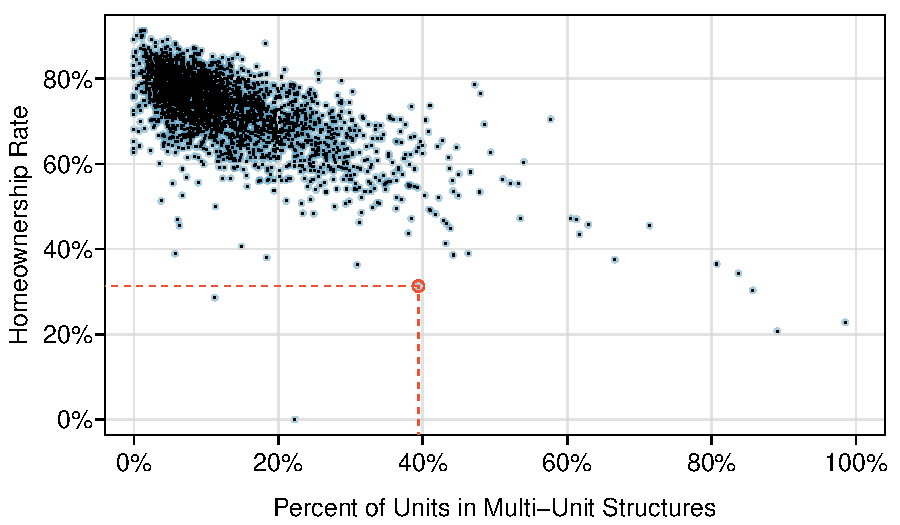
\includegraphics[width=0.8\textwidth]{ch_intro_to_data/figures/multiunitsVsOwnership/multiunitsVsOwnership}
  \caption{A scatterplot of homeownership versus the percent
      of units that are in multi-unit structures for US counties.
      The highlighted dot represents Chattahoochee County, Georgia,
      which has a multi-unit rate of 39.4\% and a homeownership rate
      of 31.3\%.}
  \label{multiunitsVsOwnership}
\end{figure}

\begin{exercise}
Examine the variables in the \data{loan50} data set,
which are described in Table~\vref{loan50Variables}.
Create two questions about possible relationships
between variables in this data set that are of interest
to you.\footnote{Two example questions: \\
  (1)~What is the relationship between loan amount and total income? \\
  (2)~If someone's income is above the average, will their
    interest rate tend to be above or below the average?}
\end{exercise}

The multi-unit and homeownership rates are said to be
associated because the plot shows a discernible pattern.
When two variables show some connection with one another,
they are called \term{associated} variables.
Associated variables can also be called \term{dependent}
variables and vice-versa.

\begin{example}{This example examines the relationship
    between population change over a 7~year period and
    median household income,
    which is visualized as a scatterplot in
    Figure~\ref{pop_change_v_med_income}.
    Are these variables associated?}
  The larger the median household income for a county,
  the higher the population growth observed for the county.
  While this trend isn't true for every county,
  the trend in the plot is evident.
  Since there is some relationship between the variables,
  they are associated.
\end{example}

%When two variables show some connection with one another,
%they are called \term{associated} variables.
%Associated variables can also be called \term{dependent}
%variables and vice-versa.
%When the variables increase together,
%as they do in Figure~\ref{loan_amount_vs_income},
%they are said to be \term{positively associated}.
%When the trend in the scatterplot goes down to the right,
%then they are described as \term{negatively correlated}.

%While we may find it interesting to consider the relationship
%between two variables such as those in the scatterplot,
%the relationship between those variables can be more complex.
%For example, interest rates on loans tend to be chosen based
%on the riskiness of the loan, i.e. how likely it is to be
%paid back, and that is likely to depend on a variety of
%details, such as what the loan is for, the person's
%creditworthiness, whether their income is verified, etc.
%We will begin exploring some of these more complex relationships
%in graphs in Chapter~\ref{ch_summarizing_data} and beyond.
%\Comment{Revise if we don't add these more rich plots...}

%\begin{example}{Figure~\ref{interest_rate_vs_loan_amount}
%    features a scatterplot of interest rate against loan amount.
%    Are these variables associated?}
%  There isn't an evident trend in the data,
%  so we would say these two variables are not associated.
%\end{example}

\begin{figure}
\centering
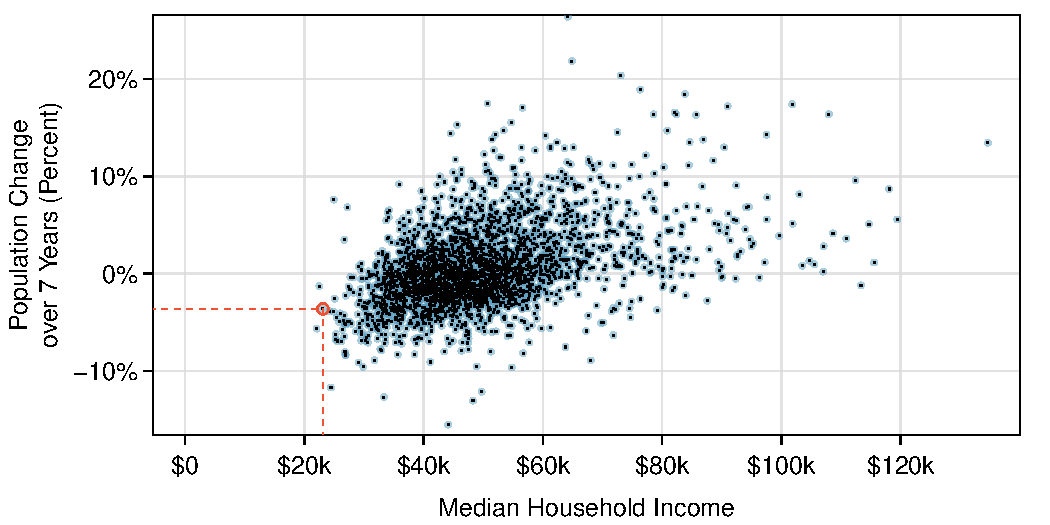
\includegraphics[width=0.8\textwidth]{ch_intro_to_data/figures/pop_change_v_med_income/pop_change_v_med_income}
\caption{A scatterplot showing
    \var{pop\_\hspace{0.3mm}change}
    against \var{median\_\hspace{0.3mm}hh\_\hspace{0.3mm}income}.
    Owsley County of Kentucky, with a poverty rate of 45.2\%
    and median household income of \$23,115, is highlighted.}
\label{pop_change_v_med_income}
\end{figure}

Because there is a downward trend in
Figure~\ref{multiunitsVsOwnership} --
counties with more units in multi-unit structures
are associated with lower homeownership --
these variables are said to be
\termsub{negatively associated}{negative association}.
A~\term{positive association} is shown in the relationship
between the
\var{median\_\hspace{0.3mm}hh\_\hspace{0.3mm}income}
and \var{pop\_\hspace{0.3mm}change}
variables represented in Figure~\ref{pop_change_v_med_income},
where counties with higher median household income tend
to have higher rates of population growth.

%\begin{figure}
%\centering
%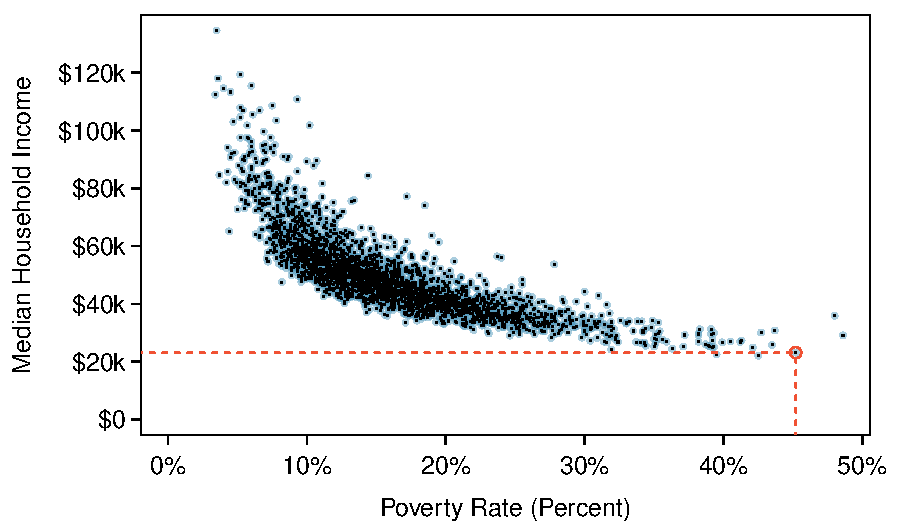
\includegraphics[width=0.8\textwidth]{ch_intro_to_data/figures/medianHHIncomePoverty/medianHHIncomePoverty}
%\caption{A scatterplot showing
%    \var{median\_\hspace{0.3mm}hh\_\hspace{0.3mm}income}
%    against \var{poverty}.
%    Owsley County of Kentucky, with a poverty rate of 45.2\%
%    and median household income of \$23,115, is highlighted.}
%\label{medianHHIncomePoverty}
%\end{figure}

%Because there is a slight downward trend in
%Figure~\ref{interest_rate_vs_income} -- counties with more units in multi-unit structures are associated with lower homeownership -- these variables are said to be \termsub{negatively associated}{negative association}. A \term{positive association} is shown in the relationship between the \var{poverty} and \var{fed\_\hspace{0.3mm}spend} variables represented in Figure~\ref{interest_rate_vs_income}, where counties with higher poverty rates tend to receive more federal spending per capita.

If two variables are not associated,
then they are said to be \term{independent}.
That is, two variables are independent if there
is no evident relationship between the two.

\begin{termBox}{\tBoxTitle{Associated or independent, not both}
A pair of variables are either related in some way (associated) or not (independent). No pair of variables is both associated and independent.}
\end{termBox}

\index{data!county|)}


%%%%%
\section[Overview of data collection principles]{Overview of data collection principles \sectionvideohref{youtube-2N_bkiyTiXU&list=PLkIselvEzpM6pZ76FD3NoCvvgkj_p-dE8} \sectionslideshref{gdoc_os3_slides_1-3}}
\label{overviewOfDataCollectionPrinciples}

\index{sample|(}
\index{population|(}

The first step in conducting research is to identify topics or questions that are to be investigated. A clearly laid out research question is helpful in identifying what subjects or cases should be studied and what variables are important. It is also important to consider \emph{how} data are collected so that they are reliable and help achieve the research goals.

\subsection{Populations and samples}
\label{populationsAndSamples}

Consider the following three research questions:
\begin{enumerate}
\setlength{\itemsep}{0mm}
\item What is the average mercury content in swordfish in the Atlantic Ocean?
\item\label{timeToGraduationQuestionForUCLAStudents} Over the last 5 years, what is the average time to complete a degree for Duke undergraduate students?
\item\label{identifyPopulationOfStentStudy} Does a new drug reduce the number of deaths in patients with severe heart disease?
\end{enumerate}
Each research question refers to a target \term{population}. In the first question, the target population is all swordfish in the Atlantic ocean, and each fish represents a case. Often times, it is too expensive to collect data for every case in a population. Instead, a sample is taken. A \term{sample} represents a subset of the cases and is often a small fraction of the population. For instance, 60 swordfish (or some other number) in the population might be selected, and this sample data may be used to provide an estimate of the population average and answer the research question.

\begin{exercise} \label{identifyingThePopulationForTwoQuestionsInPopAndSampSubsection}
For the second and third questions above, identify the target population and what represents an individual case.\footnote{(\ref{timeToGraduationQuestionForUCLAStudents}) Notice that the first question is only relevant to students who complete their degree; the average cannot be computed using a student who never finished her degree. Thus, only Duke undergraduate students who have graduated in the last five years represent cases in the population under consideration. Each such student would represent an individual case. (\ref{identifyPopulationOfStentStudy}) A person with severe heart disease represents a case. The population includes all people with severe heart disease.}
\end{exercise}


\subsection{Anecdotal evidence}
\label{anecdotalEvidenceSubsection}

Consider the following possible responses to the three research questions:
\begin{enumerate}
\item A man on the news got mercury poisoning from eating swordfish, so the average mercury concentration in swordfish must be dangerously high.
\item\label{iKnowThreeStudentsWhoTookMoreThan7YearsToGraduateAtDuke} I met two students who took more than 7 years to graduate from Duke, so it must take longer to graduate at Duke than at many other colleges.
\item\label{myFriendsDadDiedAfterSulphinpyrazon} My friend's dad had a heart attack and died after they gave him a new heart disease drug, so the drug must not work.
\end{enumerate}
Each conclusion is based on data. However, there are two problems. First, the data only represent one or two cases. Second, and more importantly, it is unclear whether these cases are actually representative of the population. Data collected in this haphazard fashion are called \term{anecdotal evidence}.

\setlength{\captionwidth}{\textwidth-80mm}
\begin{figure}
\centering
\hspace{8mm}\includegraphics[width=55mm]{ch_intro_to_data/figures/mnWinter/mnWinter}\hspace{4mm}
\begin{minipage}[b]{\textwidth - 80mm}
   \caption[anecdotal evidence]{In February 2010, some media pundits cited one large snow storm as valid evidence against global warming. As comedian Jon Stewart pointed out, ``It's one storm, in one region, of one country.''
   \label{mnWinter}}
\end{minipage}
\end{figure}
\setlength{\captionwidth}{\mycaptionwidth}

\begin{termBox}{\tBoxTitle{Anecdotal evidence}
Be careful of data collected in a haphazard fashion. Such evidence may be true and verifiable, but it may only represent extraordinary cases.}
\end{termBox}

Anecdotal evidence typically is composed of unusual cases that we recall based on their striking characteristics. For instance, we are more likely to remember the two people we met who took 7 years to graduate than the six others who graduated in four years. Instead of looking at the most unusual cases, we should examine a sample of many cases that represent the population.

\subsection{Sampling from a population}

\index{sample!random sample|(}

We might try to estimate the time to graduation for Duke undergraduates in the last 5 years by collecting a sample of students. All graduates in the last 5 years represent the \emph{population}\index{population}, and graduates who are selected for review are collectively called the \emph{sample}\index{sample}. In general, we always seek to \emph{randomly} select a sample from a population. The most basic type of random selection is equivalent to how raffles are conducted. For example, in selecting graduates, we could write each graduate's name on a raffle ticket and draw 100 tickets. The selected names would represent a random sample of 100 graduates.

\begin{figure}[ht]
\centering
\includegraphics[width=0.47\textwidth]{ch_intro_to_data/figures/popToSample/popToSampleGraduates}
\caption{In this graphic, five graduates are randomly selected from the population to be included in the sample.}
\label{popToSampleGraduates}
\end{figure}

Why pick a sample randomly? Why not just pick a sample by hand? Consider the following scenario.

\begin{example}{Suppose we ask a student who happens to be majoring in nutrition to select several graduates for the study. What kind of students do you think she might collect? Do you think her sample would be representative of all graduates?}
Perhaps she would pick a disproportionate number of graduates from health-related fields. Or perhaps her selection would be well-representative of the population. When selecting samples by hand, we run the risk of picking a \emph{biased} sample, even if that bias is unintentional or difficult to discern.
\end{example}

\begin{figure}
\centering
\includegraphics[width=0.47\textwidth]{ch_intro_to_data/figures/popToSample/popToSubSampleGraduates}
\caption{Instead of sampling from all graduates equally, a nutrition major might inadvertently pick graduates with health-related majors disproportionately often.}
\label{popToSubSampleGraduates}
\end{figure}

If someone was permitted to pick and choose exactly which graduates were included in the sample, it is entirely possible that the sample could be skewed to that person's interests, which may be entirely unintentional. This introduces \term{bias} into a sample. Sampling randomly helps resolve this problem. The most basic random sample is called a \term{simple random sample}, and which is equivalent to using a raffle to select cases. This means that each case in the population has an equal chance of being included and there is no implied connection between the cases in the sample.

\APVersion{Sometimes a simple random sample is difficult to implement and an alternative method is helpful. One such substitute is a \term{systematic sample}, where one case is sampled after letting a fixed number of others, say 10 other cases, pass by. Since this approach uses a mechanism that is not easily subject to personal biases, it often yields a reasonably representative sample. This book will focus on random samples since the use of systematic samples is uncommon and requires additional considerations of the context.}{}

The act of taking a simple random sample helps minimize bias. However, bias can crop up in other ways.
Even when people are picked at random, e.g. for surveys, caution must be exercised if the \term{non-response} \index{sample!non-response|textbf} is high. For instance, if only 30\% of the people randomly sampled for a survey actually respond, then it is unclear whether the results are \term{representative} of the entire population. This \term{non-response bias} \index{sample!non-response bias|textbf} can skew results.

\begin{figure}[h]
\centering
\includegraphics[width=0.5\textwidth]{ch_intro_to_data/figures/popToSample/surveySample}
\caption{Due to the possibility of non-response, surveys studies may only reach a certain group within the population. It is difficult, and often times impossible, to completely fix this problem.}
\label{surveySample}
\end{figure}

Another common downfall is a \term{convenience sample}\index{sample!convenience sample}, where individuals who are easily accessible are more likely to be included in the sample. For instance, if a political survey is done by stopping people walking in the Bronx, this will not represent all of New York City. It is often difficult to discern what sub-population a convenience sample represents.

\begin{exercise}
We can easily access ratings for products, sellers, and companies through websites. These ratings are based only on those people who go out of their way to provide a rating. If 50\% of online reviews for a product are negative, do you think this means that 50\% of buyers are dissatisfied with the product?\footnote{Answers will vary. From our own anecdotal experiences, we believe people tend to rant more about products that fell below expectations than rave about those that perform as expected. For this reason, we suspect there is a negative bias in product ratings on sites like Amazon. However, since our experiences may not be representative, we also keep an open mind.}
\end{exercise}

\index{sample!random sample|)}
\index{population|)}
\index{sample|)}

\subsection{Explanatory and response variables}
\label{explanatoryAndResponse}

\Comment{This subsection was significantly updated.}

\index{data!county|(}

Consider the following question from
page~\pageref{pop_change_v_median_hh_income_question}
for the \data{county} data set:
\begin{enumerate}
\item[(2)]
    Does county population change tend to correspond to an increase
    or decrease for counties with higher median household incomes?
\end{enumerate}
If we suspect a county's median household income might affect
its growth rate,
then median household income is the
\termsub{explanatory}{explanatory variable}
variable and the change in the population is the
\termsub{response}{response variable} variable in the
relationship.\footnote{Sometimes the term
\term{independent variable} is used for
the explanatory variable and \term{dependent variable} for
the response variable.
However, because this is confusing since a \emph{pair} of
variables might be independent or dependent, we avoid this
particular terminology.}
If there are many variables, it is possible to consider
a number of them as explanatory variables.

\index{data!county|)}

\begin{termBox}{\tBoxTitle{Explanatory and response variables}
When we suspect one variable might causally affect another,
we label the first variable the explanatory variable and the
second the response variable.
\vspace{1mm}

\hspace{10mm}\includegraphics[height=0.34in]{ch_intro_to_data/figures/expResp/expResp}

Often times it doesn't seem that one variable might affect the other,
in which case these labels should not be applied.}
\end{termBox}

The explanatory and response labels only considers
a \emph{suspected} causal relationship, and it does not guarantee
that such a causal relationship exists.
Evaluating whether the relationship is in fact causal
requires an experiment.


\subsection{Introducing observational studies and experiments}

There are two primary types of data collection: observational studies and experiments.

Researchers perform an \term{observational study} when they collect data in a way that does not directly interfere with how the data arise. For instance, researchers may collect information via surveys, review medical or company records, or follow a \term{cohort} of many similar individuals to study why certain diseases might develop. In each of these situations, researchers merely observe the data that arise. In general, observational studies can provide evidence of a naturally occurring association between variables, but they cannot by themselves show a causal connection.

When researchers want to investigate the possibility of a causal connection, they conduct an \term{experiment}. Usually there will be both an explanatory and a response variable. For instance, we may suspect administering a drug will reduce mortality in heart attack patients over the following year. To check if there really is a causal connection between the explanatory variable and the response, researchers will collect a sample of individuals and split them into groups. The individuals in each group are \emph{assigned} a treatment. When individuals are randomly assigned to a group, the experiment is called a \term{randomized experiment}. For example, each heart attack patient in the drug trial could be randomly assigned,  perhaps by flipping a coin, into one of two groups: the first group receives a \term{placebo} (fake treatment) and the second group receives the drug. See the case study in Section~\ref{basicExampleOfStentsAndStrokes} for another example of an experiment, though that study did not employ a placebo.

\begin{tipBox}{\tipBoxTitle{association $\neq$ causation}
In general, association does not imply causation, and causation can only be inferred from a randomized experiment.}
\end{tipBox}


%%%%%
\section[Observational studies and sampling strategies]{Observational studies \\and sampling strategies \sectionvideohref{youtube-KyuaX10l3GQ&list=PLkIselvEzpM6pZ76FD3NoCvvgkj_p-dE8}~\sectionslideshref{gdoc_os3_slides_1-4}}

\subsection{Observational studies}

Generally, data in observational studies are collected only by monitoring what occurs, while experiments require the primary explanatory variable in a study be assigned for each subject by the researchers.

Making causal conclusions based on experiments is often reasonable. However, making the same causal conclusions based on observational data can be treacherous and is not recommended. Thus, observational studies are generally only sufficient to show associations.

\begin{exercise} \label{sunscreenLurkingExample}
Suppose an observational study tracked sunscreen use and skin cancer, and it was found that the more sunscreen someone used, the more likely the person was to have skin cancer. Does this mean sunscreen \emph{causes} skin cancer?\footnote{No. See the paragraph following the exercise for an explanation.}
\end{exercise}

Some previous research tells us that using sunscreen actually reduces skin cancer risk, so maybe there is another variable that can explain this hypothetical association between sunscreen usage and skin cancer. One important piece of information that is absent is sun exposure. If someone is out in the sun all day, she is more likely to use sunscreen \emph{and} more likely to get skin cancer. Exposure to the sun is unaccounted for in the simple investigation.
\begin{center}
\includegraphics[height=1.0in]{ch_intro_to_data/figures/variables/sunCausesCancer}
\end{center}
% Some studies:
% http://www.sciencedirect.com/science/article/pii/S0140673698121682
% http://archderm.ama-assn.org/cgi/content/abstract/122/5/537
% Study with a similar scenario to that described here:
% http://onlinelibrary.wiley.com/doi/10.1002/ijc.22745/full

Sun exposure is what is called a \term{confounding variable},\footnote{Also called a \term{lurking variable}, \term{confounding factor}, or a \term{confounder}.} which is a variable that is correlated with both the explanatory and response variables. While one method to justify making causal conclusions from observational studies is to exhaust the search for confounding variables, there is no guarantee that all confounding variables can be examined or measured.

In the same way, the \data{county} data set is an observational study with confounding variables, and its data cannot easily be used to make causal conclusions.

\begin{exercise}
Figure~\ref{multiunitsVsOwnership} shows a negative association between the homeownership rate and the percentage of multi-unit structures in a county. However, it is unreasonable to conclude that there is a causal relationship between the two variables. Suggest one or more other variables that might explain the relationship visible in Figure~\ref{multiunitsVsOwnership}.\footnote{Answers will vary. Population density may be important. If a county is very dense, then this may require a larger fraction of residents to live in multi-unit structures. Additionally, the high density may contribute to increases in property value, making homeownership infeasible for many residents.}
\end{exercise}

Observational studies come in two forms: prospective and retrospective studies. A \term{prospective study} identifies individuals and collects information as events unfold. For instance, medical researchers may identify and follow a group of similar individuals over many years to assess the possible influences of behavior on cancer risk. One example of such a study is The Nurses' Health Study, started in 1976 and expanded in 1989.\footnote{\oiRedirect{textbook-channing_nurse_study}{www.channing.harvard.edu/nhs}} This prospective study recruits registered nurses and then collects data from them using questionnaires. \termsub{Retrospective studies}{retrospective studies} collect data after events have taken place, e.g. researchers may review past events in medical records. Some data sets, such as \data{county}, may contain both prospectively- and retrospectively-collected variables. Local governments prospectively collect some variables as events unfolded (e.g. retails sales) while the federal government retrospectively collected others during the 2010 census (e.g. county population counts).

\subsection{Four sampling methods (special topic)}
\label{fourSamplingMethods}
\label{threeSamplingMethods}

Almost all statistical methods are based on the notion of implied randomness. If observational data are not collected in a random framework from a population, these statistical methods -- the estimates and errors associated with the estimates -- are not reliable. Here we consider four random sampling techniques: simple, stratified, cluster, and multistage sampling. Figures~\ref{simple_stratified} and~\ref{cluster_multistage} provide graphical representations of these techniques.

\begin{figure}
\centering
\includegraphics[width=\textwidth]{ch_intro_to_data/figures/samplingMethodsFigure/simple_stratified}
\caption{Examples of simple random\index{sample!simple random sampling} and stratified sampling\index{sample!stratified sampling}. In the top panel, simple random sampling was used to randomly select the 18 cases. In the bottom panel, stratified sampling was used: cases were grouped into strata, then simple random sampling was employed within \mbox{each stratum}.}
\label{simple_stratified}
\end{figure}

\termsub{Simple random sampling}{sample!simple random sampling} is probably the most intuitive form of random sampling. Consider the salaries of Major League Baseball (MLB) players, where each player is a member of one of the league's 30 teams. To take a simple random sample of 120 baseball players and their salaries from the 2010 season, we could write the names of that season's 828 players onto slips of paper, drop the slips into a bucket, shake the bucket around until we are sure the names are all mixed up, then draw out slips until we have the sample of 120 players. In general, a sample is referred to as ``simple random'' if each case in the population has an equal chance of being included in the final sample \emph{and} knowing that a case is included in a sample does not provide useful information about which other cases are included.

\termsub{Stratified sampling}{sample!stratified sampling} is a divide-and-conquer sampling strategy. The population is divided into groups called \term{strata}\index{sample!strata|textbf}. The strata are chosen so that similar cases are grouped together, then a second sampling method, usually simple random sampling, is employed within each stratum. In the baseball salary example, the teams could represent the strata, since some teams have a lot more money (up to 4~times as much!). Then we might randomly sample 4 players from each team for a total of 120 players.

Stratified sampling is especially useful when the cases in each stratum are very similar with respect to the outcome of interest. The downside is that analyzing data from a stratified sample is a more complex task than analyzing data from a simple random sample. The analysis methods introduced in this book would need to be extended to analyze data collected using stratified sampling.

\begin{example}{Why would it be good for cases within each stratum to be very similar?}
We might get a more stable estimate for the subpopulation in a stratum if the cases are very similar. These improved estimates for each subpopulation will help us build a reliable estimate for the full population.
\end{example}

In a \termsub{cluster sample}{sample!cluster sample}, we break up the population into many groups, called \termsub{clusters}{sample!cluster}. Then we sample a fixed number of clusters and include all observations from each of those clusters in the sample. A \termsub{multistage sample}{sample!multistage sample} is like a cluster sample, but rather than keeping all observations in each cluster, we collect a random sample within each selected cluster. %Multistage sampling is similar to stratified sampling in its process, except that stratified sampling requires observations be sampled from \emph{every} stratum.

\begin{figure}
\centering
\includegraphics[width=\textwidth]{ch_intro_to_data/figures/samplingMethodsFigure/cluster_multistage}
\caption{Examples of cluster\index{sample!cluster sampling} and multistage sampling\index{sample!multistage sampling}. In the top panel, cluster sampling was used. Here, data were binned into nine clusters, three of these clusters were sampled, and all observations within these three cluster were included in the sample. In the bottom panel, multistage sampling was used.
It differs from cluster sampling in that of the clusters selected, we randomly select a subset of each cluster to be included in the sample.}
\label{cluster_multistage}
\end{figure}

Sometimes cluster or multistage sampling can be more economical than the alternative sampling techniques. Also, unlike stratified sampling, these approaches are most helpful when there is a lot of case-to-case variability within a cluster but the clusters themselves don't look very different from one another. For example, if neighborhoods represented clusters, then cluster or multistage sampling work best when the neighborhoods are very diverse. A downside of these methods is that more advanced analysis techniques are typically required, though the methods in this book can be extended to handle such data.

\begin{example}{Suppose we are interested in estimating the malaria rate in a densely tropical portion of rural Indonesia. We learn that there are 30 villages in that part of the Indonesian jungle, each more or less similar to the next. Our goal is to test 150 individuals for malaria. What sampling method should be employed?}
A simple random sample would likely draw individuals from all 30 villages, which could make data collection extremely expensive. Stratified sampling would be a challenge since it is unclear how we would build strata of similar individuals. However, cluster sampling or multistage sampling seem like very good ideas. If we decided to use multistage sampling, we might randomly select half of the villages, then randomly select 10 people from each. This would probably reduce our data collection costs substantially in comparison to a simple random sample, and this approach would still give us reliable information.
\end{example}


%%%%%
\section[Experiments]{Experiments \sectionvideohref{youtube-g7JGe_ykB3I&list=PLkIselvEzpM6pZ76FD3NoCvvgkj_p-dE8}~\sectionslideshref{gdoc_os3_slides_1-5}}
\label{experimentsSection}

Studies where the researchers assign treatments to cases are called \termsub{experiments}{experiment}. When this assignment includes randomization, e.g.~using a coin flip to decide which treatment a patient receives, it is called a \term{randomized experiment}. Randomized experiments are fundamentally important when trying to show a causal connection between two variables.

\subsection{Principles of experimental design}
\label{experimentalDesignPrinciples}

Randomized experiments are generally built on four principles.
\begin{description}
\item[Controlling.] Researchers assign treatments to cases, and they do their best to \term{control} any other differences in the groups. For example, when patients take a drug in pill form, some patients take the pill with only a sip of water while others may have it with an entire glass of water. To control for the effect of water consumption, a doctor may ask all patients to drink a 12 ounce glass of water with the pill.
\item[Randomization.] Researchers randomize patients into treatment groups to account for variables that cannot be controlled. For example, some patients may be more susceptible to a disease than others due to their dietary habits. Randomizing patients into the treatment or control group helps even out such differences, and it also prevents accidental bias from entering the study.
\item[Replication.] The more cases researchers observe, the more accurately they can estimate the effect of the explanatory variable on the response. In a single study, we \term{replicate} by collecting a sufficiently large sample. Additionally, a group of scientists may replicate an entire study to verify an earlier finding.

\begin{figure}
\centering
\includegraphics[width=0.78\textwidth]{ch_intro_to_data/figures/figureShowingBlocking/figureShowingBlocking}
\caption{Blocking using a variable depicting patient risk. Patients are first divided into low-risk and high-risk blocks, then each block is evenly separated into the treatment groups using randomization. This strategy ensures an equal representation of patients in each treatment group from both the low-risk and high-risk categories.}
\label{figureShowingBlocking}
\end{figure}

\item[Blocking.] Researchers sometimes know or suspect that variables, other than the treatment, influence the response. Under these circumstances, they may first group individuals based on this variable into \term{blocks} and then randomize cases within each block to the treatment groups. This strategy is often referred to as \term{blocking}. For instance, if we are looking at the effect of a drug on heart attacks, we might first split patients in the study into low-risk and high-risk blocks, then randomly assign half the patients from each block to the control group and the other half to the treatment group, as shown in Figure~\ref{figureShowingBlocking}. This strategy ensures each treatment group has an equal number of low-risk and high-risk patients.
\end{description}

It is important to incorporate the first three experimental design principles into any study, and this book describes applicable methods for analyzing data from such experiments. Blocking is a slightly more advanced technique, and statistical methods in this book may be extended to analyze data collected using blocking.

\subsection{Reducing bias in human experiments}
\label{biasInHumanExperiments}

Randomized experiments are the gold standard for data collection, but they do not ensure an unbiased perspective into the cause and effect relationships in all cases. Human studies are perfect examples where bias can unintentionally arise. Here we reconsider a study where a new drug was used to treat heart attack patients.\footnote{Anturane Reinfarction Trial Research Group. 1980. Sulfinpyrazone in the prevention of sudden death after myocardial infarction. New England Journal of Medicine 302(5):250-256.} In particular, researchers wanted to know if the drug reduced deaths in patients.

These researchers designed a randomized experiment because they wanted to draw causal conclusions about the drug's effect. Study volunteers\footnote{Human subjects are often called \term{patients}, \term{volunteers}, or \term{study participants}.} were randomly placed into two study groups. One group, the \term{treatment group}, received the drug. The other group, called the \term{control group}, did not receive any drug treatment.

Put yourself in the place of a person in the study. If you are in the treatment group, you are given a fancy new drug that you anticipate will help you. On the other hand, a person in the other group doesn't receive the drug and sits idly, hoping her participation doesn't increase her risk of death. These perspectives suggest there are actually two effects: the one of interest is the effectiveness of the drug, and the second is an emotional effect that is difficult to quantify.

Researchers aren't usually interested in the emotional effect, which might bias the study. To circumvent this problem, researchers do not want patients to know which group they are in. When researchers keep the patients uninformed about their treatment, the study is said to be \term{blind}. But there is one problem: if a patient doesn't receive a treatment, she will know she is in the control group. The solution to this problem is to give fake treatments to patients in the control group. A fake treatment is called a \term{placebo}, and an effective placebo is the key to making a study truly blind. A classic example of a placebo is a sugar pill that is made to look like the actual treatment pill. Often times, a placebo results in a slight but real improvement in patients. This effect has been dubbed the \term{placebo~effect}.

The patients are not the only ones who should be blinded: doctors and researchers can accidentally bias a study. When a doctor knows a patient has been given the real treatment, she might inadvertently give that patient more attention or care than a patient that she knows is on the placebo. To guard against this bias, which again has been found to have a measurable effect in some instances, most modern studies employ a \term{double-blind} setup where doctors or researchers who interact with patients are, just like the patients, unaware of who is or is not receiving the treatment.\footnote{There are always some researchers involved in the study who do know which patients are receiving which treatment. However, they do not interact with the study's patients and do not tell the blinded health care professionals who is receiving which treatment.}

\begin{exercise}
Look back to the study in Section~\ref{basicExampleOfStentsAndStrokes} where researchers were testing whether stents were effective at reducing strokes in at-risk patients. Is this an experiment? Was the study blinded? Was it double-blinded?\footnote{The researchers assigned the patients into their treatment groups, so this study was an experiment. However, the patients could distinguish what treatment they received, so this study was not blind. The study could not be double-blind since it was not blind.}
\end{exercise}


